\documentclass[11pt]{article}
\usepackage[margin=1in]{geometry}
\usepackage[T1]{fontenc}
\usepackage{lmodern}
\usepackage{microtype}
\usepackage{amsmath,amssymb}
\usepackage{booktabs,tabularx,array}
\usepackage{enumitem}
\usepackage{xcolor}
\usepackage{listings}
\usepackage{tikz}
\usetikzlibrary{arrows.meta,positioning}
\usepackage[obeyspaces,spaces]{url}
\usepackage[hidelinks]{hyperref}

\setlist{itemsep=2pt,topsep=4pt}
\setlength{\parskip}{5pt}
\setlength{\parindent}{0pt}
\setlength{\emergencystretch}{3em}
\renewcommand{\arraystretch}{1.25}
\newcolumntype{Y}{>{\raggedright\arraybackslash}X}

\definecolor{codebg}{RGB}{247,247,250}
\definecolor{codeframe}{RGB}{200,200,210}
\definecolor{keyword}{RGB}{30,60,140}
\definecolor{comment}{RGB}{100,110,120}
\definecolor{string}{RGB}{150,60,20}
\definecolor{notebg}{RGB}{238,244,252}
\definecolor{okbg}{RGB}{232,246,234}
\definecolor{warnbg}{RGB}{253,240,232}
\definecolor{linkc}{RGB}{20,80,170}
\definecolor{lapi}{RGB}{225,238,252}
\definecolor{leng}{RGB}{230,245,232}
\definecolor{lms4}{RGB}{252,243,224}
\definecolor{lcore}{RGB}{238,238,238}
\hypersetup{colorlinks=true,linkcolor=linkc,urlcolor=linkc,filecolor=linkc}

\lstdefinestyle{java}{language=Java, basicstyle=\ttfamily\small, columns=fullflexible, keepspaces=true,
  keywordstyle=\color{keyword}\bfseries, commentstyle=\color{comment}\itshape, stringstyle=\color{string},
  backgroundcolor=\color{codebg}, frame=single, rulecolor=\color{codeframe}, breaklines=true,
  showstringspaces=false, xleftmargin=4pt, xrightmargin=4pt, aboveskip=6pt, belowskip=6pt}
\lstset{style=java}

\newcommand{\code}[1]{\texttt{#1}}
\newcommand{\shadedbox}[3]{\par\smallskip\noindent\colorbox{#1}{\parbox{\dimexpr\linewidth-2\fboxsep}{\textbf{#2}\par #3}}\par\smallskip}
\newcommand{\takeaway}[1]{\shadedbox{okbg}{In short}{#1}}
\newcommand{\note}[1]{\shadedbox{notebg}{Note}{#1}}
\newcommand{\decision}[1]{\shadedbox{warnbg}{Decision needed}{#1}}
\newcommand{\docsdir}{../}
\def\thisdoc{report}
% Shared cross-document links for the ParaDEVS documents. Each document defines \docsdir (path from its folder to
% docs/) and \thisdoc (its key below), then \input's this file.
%
% \doclink{path relative to docs/}{text}: a link to another PDF. Links are plain URI actions (file:///...), because
% Edge, Chrome and VS Code's PDF viewers ignore hyperref's usual "open another PDF" (GoToR) links. The absolute
% address comes from docroot.tex, which scripts/build_docs.sh regenerates; rerun it if the folder moves.
%
% \relateddocs: the "ParaDEVS documents" box listing every document, with the current one marked.
\InputIfFileExists{\docsdir docroot.tex}{}{\gdef\docroot{.}}
\providecommand{\thisdoc}{}
\definecolor{pdlink}{RGB}{20,80,170}
\definecolor{pdrelbg}{RGB}{243,246,252}
\definecolor{pdrelframe}{RGB}{190,200,220}
\makeatletter
\newcommand{\doclink}[2]{\hyper@linkurl{\textcolor{pdlink}{\textbf{#2}}}{\docroot/#1}}
\newcommand{\pd@item}[4]{% key, path, title, description
  \def\pd@key{#1}%
  \item \ifx\pd@key\thisdoc\textbf{#3} (this document)\else\doclink{#2}{#3}\fi: #4}
\newcommand{\relateddocs}{\par\medskip\noindent
  \fcolorbox{pdrelframe}{pdrelbg}{\parbox{\dimexpr\linewidth-2\fboxsep-2\fboxrule}{\small
  \textbf{ParaDEVS documents.} The entry point is \doclink{ParaDEVS_Start_Here.pdf}{Start Here}, a reading guide
  that links every document.
  \begin{itemize}[leftmargin=1.4em,itemsep=0pt,topsep=2pt]
  \pd@item{report}{report/ParaDEVS_Build_Report.pdf}{Build Report}{what has been built, how it was verified, what is next}
  \pd@item{howto}{howto/ParaDEVS_HowTo.pdf}{How-To Guide}{setup, tutorials, API reference, troubleshooting}
  \pd@item{architecture}{architecture/ParaDEVS_Architecture.pdf}{Architecture Guide}{how the library works and how to read results}
  \pd@item{rl}{rl/ParaDEVS_RL_Plan.pdf}{RL Plan}{reinforcement-learning plan, analysis and results}
  \pd@item{control}{rl/ParaDEVS_Control_Spec.pdf}{Control Spec}{action selection: Para.decide, graph-mode planning, value and policy iteration}
  \pd@item{hybrid}{rl/ParaDEVS_Hybrid_Study.pdf}{Hybrid Study}{which draws to enumerate or sample, and how cost grows with lookahead}
  \pd@item{fastcopy}{engine/ParaDEVS_FastCopy_Proposal.pdf}{Fast-Copy Proposal}{why the engine replays steps, where time goes, how to speed it up}
  \end{itemize}}}\par\medskip}
\makeatother


\title{\textbf{ParaDEVS Library}\\[4pt]\large Build Report: what has been built so far, and how we know it works}
\author{ParaDEVS Library workspace, Binghamton}
\date{October 11, 2026 \quad (covers work from October 9--11, 2026)}

\begin{document}
\maketitle

\begin{center}
\begin{minipage}{0.88\linewidth}\small
\textbf{How to read this report.} Page~\pageref{sec:glance} is a one-page summary; if you read nothing else, read
that. Every later section opens with a green ``In short'' box, so you can skim by reading only those boxes. Terms are
defined in the glossary (Appendix~\ref{app:glossary}). The other documents are linked by name.
\end{minipage}
\end{center}

\relateddocs

\tableofcontents
\newpage

%=====================================================================
\section{At a glance}\label{sec:glance}

\begin{tabularx}{\linewidth}{@{}>{\bfseries\raggedright\arraybackslash}p{3.6cm}Y@{}}
\toprule
What it is & A Java library that runs an ordinary stochastic MS4 DEVS model as a \emph{paratemporal} computation:
  each time the model makes a random choice, the engine follows the possible outcomes, weights them, and returns the
  exact (or sampled) distribution of what you asked it to observe.\\
What a model must do & One thing: get every random value from \code{Para.choose(label, law)} instead of a random
  number generator. Nothing else in the model changes, and it still runs in plain MS4.\\
Does it work? & \textbf{Yes. 77 of 77 checks pass} against three independent references: the paper's worked example
  (exact match), the Demo Deliverable finance run (to $10^{-12}$), and the original baseball engine (to $10^{-12}$).\\
Speed-up from merging & Baseball, 6 plate appearances: 24{,}450 leaves in 17.4\,s without merging, 195 outcomes in
  0.65\,s with safe merging. Same answer.\\
Documentation & How-to guide with two tutorials (17 pp), architecture guide (13 pp), RL plan with results (9 pp),
  and this report.\\
Working environment & VS Code, preconfigured: one task builds and runs every test.\\
RL track & Setup done; Python can drive the Java engine. First studies: the paratemporal ``exact'' target roughly
  \textbf{halves the learning error per real episode} compared with standard n-step TD.\\
Next & Finish the Python prototypes (control, hybrid selection), then add RL features to the Java library and a
  Gymnasium wrapper for Python.\\
\bottomrule
\end{tabularx}

\decision{Should the Java library get an \emph{expectation-only} merge as an opt-in? It is much cheaper for RL
targets, but it keeps only averages (not full distributions), which goes beyond the ``safe merging only'' rule you
set. It is used only in the Python prototypes so far. Details in Section~\ref{sec:next}.}

%=====================================================================
\section{Starting point}\label{sec:before}

\takeaway{The old paratemporal engines worked, but only for one model shape, with the tree logic and domain code
mixed together. The goal was a general library built on the theory in \path{Do s/documents/paratemporal}.}

What existed on October 9:
\begin{itemize}
\item \textbf{Three copies of one hand-written engine}: Baseball v7, Finance v4-IH and the Demo Deliverable. Only the
  Demo Deliverable compiled and ran as-is; Finance v4-IH has an empty \code{CallGenerator.java}.
\item \textbf{One model shape only}: one generator feeding one state machine, one random choice per step, made at a
  known time in a known component.
\item \textbf{Workarounds in the wiring}: probabilities packed into message values, state written directly into
  models, domain code (shares, runs) inside the engine.
\item \textbf{Step and draw were the same thing}: one tree level was one forced outcome, one full simulation run and
  one state save. A model with two random choices in one event could not be expressed.
\end{itemize}

Decisions you made (October 9), which the whole build follows:
\begin{enumerate}
\item Java, on top of the MS4 DEVS core.
\item The paper's conventions: models make draws inside their own transitions; the engine branches.
\item Safe merging only (the old IH ``merge by shares'' is not in the library).
\item Verification set: timed reward (paper), finance (Demo baseline), baseball (legacy engine).
\item Version 0 scope: fixed input trace, horizon counted in events, exhaustive / Monte Carlo / partial selection.
\item \path{Do s} is the theory authority; \code{Main\_Sol\_Base} is out of scope.
\end{enumerate}

%=====================================================================
\section{What was built}\label{sec:built}

\takeaway{Three small layers on top of the unchanged MS4 core: a one-call model API, the engine from the paper, and an
adapter that drives MS4 models deterministically. About 1{,}200 lines of library code.}

\begin{center}
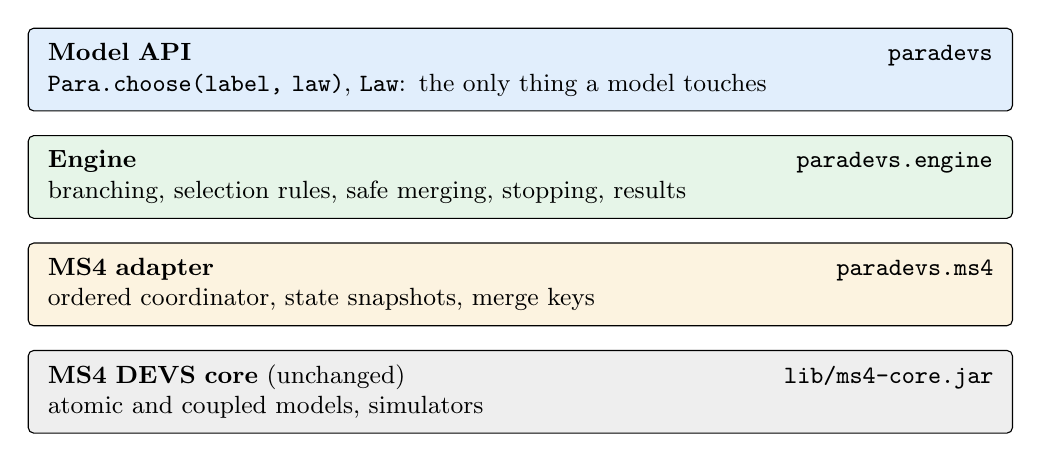
\begin{tikzpicture}[layer/.style={draw,rounded corners=2pt,minimum width=12.5cm,minimum height=1.05cm,align=left,
  font=\small,text width=12cm}]
\node[layer,fill=lapi]  (api) {\textbf{Model API} \hfill \code{paradevs}\\ \code{Para.choose(label, law)}, \code{Law}: the only thing a model touches};
\node[layer,fill=leng,below=3mm of api]  (eng) {\textbf{Engine} \hfill \code{paradevs.engine}\\ branching, selection rules, safe merging, stopping, results};
\node[layer,fill=lms4,below=3mm of eng]  (ms4) {\textbf{MS4 adapter} \hfill \code{paradevs.ms4}\\ ordered coordinator, state snapshots, merge keys};
\node[layer,fill=lcore,below=3mm of ms4] (core) {\textbf{MS4 DEVS core} (unchanged) \hfill \code{lib/ms4-core.jar}\\ atomic and coupled models, simulators};
\end{tikzpicture}
\end{center}

\subsection{How a model plugs in}
A model asks for random values like this. Under plain MS4 the call simply samples; under the engine it branches.
\begin{lstlisting}
int phase = Para.choose("phase", Law.of(0, 0.25, 1, 0.75));   // 0 w.p. 0.25, 1 w.p. 0.75
\end{lstlisting}
And an experiment runs it like this:
\begin{lstlisting}
ParaResult<X> r = ParaEngine.run(
    ParaSpec.of(() -> new MyModel(), myTransducer)  // model + what to observe
        .trace(InputTrace.builder().at(0.0, "action", "a").build())
        .horizon(5)                                 // stop after 5 events
        .selection(SelectionRule.exhaustive())      // or monteCarlo(N), ...
        .merge(ParaSpec.Merge.SAFE));
r.distribution();  r.expectation(f);  r.residual();  r.stats();
\end{lstlisting}

\subsection{The parts, in plain terms}
\begin{tabularx}{\linewidth}{@{}>{\raggedright}p{4.3cm}Y@{}}
\toprule
\textbf{Part} & \textbf{What it does}\\
\midrule
\code{Para}, \code{Law} & The model's only contact with the library. \code{Law} is a finite list of values with
  probabilities; it rejects laws whose mass is not 1 (with \code{Law.asGiven} for slightly imperfect source data).\\
\code{ParaEngine} & The algorithm from \path{main_paratemporal.tex} (main / $\Gamma_{PT}$ / Advance / doExpansion /
  RunLocal), one global clock, stopping by horizon, acceptance or passivity.\\
\code{SelectionRule} & Which outcomes to follow at each draw: all (exhaustive), a sample (Monte Carlo), only likely
  ones (partial, with the leftover mass reported as the \emph{residual}), or a mix chosen by draw label (hybrid).\\
\code{ParaSpec.Merge.SAFE} & Joins two branches only when \emph{everything} about their future is identical: full
  model state, clock, inputs still to come and the observation so far. This cannot change any answer.\\
\code{ParaResult} & The distribution, expectations, marginals, total mass, residual and run statistics.\\
\code{ModelNode} & Drives MS4 atomic models through MS4's own simulator, and coupled models through a coordinator
  that visits children in a fixed order (MS4's own does not; see Section~\ref{sec:issues}).\\
\code{Snapshots}, \code{StateKeys} & Copy a model's full state (Java serialization) and build its merge key (every
  field, by reflection, with an override hook).\\
\bottomrule
\end{tabularx}

\subsection{The one idea that makes it general: branch at the draw}
The engine branches at each \emph{draw}, not at each \emph{event}. When a model calls \code{Para.choose} and the
value is not yet known, the engine stops that event, creates one branch per outcome, and later replays the event from
the saved state with the chosen value supplied. An event with two draws therefore becomes two levels of branching,
which the old engines could not express. The architecture guide, Section ``Step versus draw'', explains this in detail.

\subsection{Examples shipped with the library}
\begin{tabularx}{\linewidth}{@{}lY@{}}
\toprule
\textbf{Example} & \textbf{What it shows}\\
\midrule
Tutorial: service line & The smallest complete model; answer checkable by hand (P(3 served) = 0.36).\\
Timed reward & The paper's worked example, with a known exact answer.\\
Finance & The Demo trader/portfolio rewritten as a plain DEVS coupled model, no engine-side domain code.\\
Baseball & The legacy batting model, same treatment.\\
Sandbox random walk & Template for new experiments (\path{src/sandbox}).\\
MS4 Me import demo & An unmodified MS4 Me-generated model (JobProcessorExample) running under the engine with two
  marked edits.\\
\bottomrule
\end{tabularx}

%=====================================================================
\section{How we know it works}\label{sec:verify}

\takeaway{Every number the old engines and the paper produce is reproduced, exactly or to $10^{-12}$. All 77 checks
pass in one command. Safe merging gives the same answers far faster.}

\subsection{Checks against independent references}
\begin{tabularx}{\linewidth}{@{}>{\raggedright}p{2.6cm}>{\raggedright}p{4.2cm}Yr@{}}
\toprule
\textbf{Test} & \textbf{Reference} & \textbf{Result} & \textbf{Checks}\\
\midrule
Tutorial & Hand calculation & P(3 served) = 0.36 exactly; Monte Carlo within 4 standard errors & 10\\
Timed reward & \path{pt_reward_enumeration.py} from the paper & Exact law (6352, 10948, 9793, 12907)/40000; 64 leaves
  and 63 choice nodes as in the paper. Merging, sampling and partial runs all consistent & 24\\
Finance & Demo Deliverable run of Oct.~9 & Share probabilities to $10^{-12}$; expected net $-38.9056847633$ vs
  $-38.9056847626$ & 28\\
Baseball & Original BaseballDEVS\_v7 engine, fresh run & All 39 (5 PA) and 55 (6 PA) states to $10^{-12}$;
  E[runs after 5 PA] = 0.315529858502410, identical & 15\\
\midrule
\multicolumn{3}{@{}l}{\textbf{Total (last run October 11, 2026)}} & \textbf{77 / 77}\\
\bottomrule
\end{tabularx}

Two more runs are part of the test script but have no numeric baseline: the sandbox random walk (binomial answer
checked) and a plain MS4 run showing that models still work without the engine.

\note{The old IH numbers (merged by shares) are recovered as \emph{marginals} of the exact distribution. That is why
the library can drop IH merging without losing any result the old engine reported.}

\subsection{What merging saves}
\begin{tabularx}{\linewidth}{@{}lYY@{}}
\toprule
\textbf{Case} & \textbf{No merging} & \textbf{Safe merging (same answer)}\\
\midrule
Timed reward & 64 leaves & 8 outcomes\\
Finance, depth 6 & 729 leaves, 0.69\,s & 288 outcomes, 0.35\,s\\
Baseball, 5 PA & 4{,}890 leaves, 4.3\,s & 145 outcomes, 0.41\,s\\
Baseball, 6 PA & 24{,}450 leaves, 17.4\,s & 195 outcomes, 0.65\,s \ (legacy engine: about 17\,s)\\
\bottomrule
\end{tabularx}

%=====================================================================
\section{Problems found and fixed}\label{sec:issues}

\takeaway{Ten real problems came up. Two were genuine design hazards (nondeterministic MS4 ordering, and merging
Monte Carlo samples). Both are now prevented in code and covered by tests.}

\begin{tabularx}{\linewidth}{@{}>{\raggedright}p{4.4cm}>{\raggedright}p{4.6cm}Y@{}}
\toprule
\textbf{Problem} & \textbf{Effect} & \textbf{Fix}\\
\midrule
MS4's coupled coordinator visits children in hash order & A replayed event could make its draws in a different
  order, silently mixing up branches & Library ships its own coordinator with a fixed visiting order\\
Monte Carlo samples + safe merging & All samples start identical, so they merged into one path: P(+6) came out 0
  instead of about 0.016 & Engine now refuses this combination with a clear message; test added\\
Baseball source data sums to 1.0004 (Machado's row) & Strict law check rejected the legacy data &
  \code{Law.asGiven(\dots, 10\textsuperscript{-3})} for imperfect source data\\
Legacy baseball kept zero-probability states & State counts differed from the old engine & Compare
  positive-probability states only (the paper drops zero-weight branches)\\
Test helper compared \code{Long} with \code{Integer} & False failures & Compare numerically\\
Build script ignored compile errors & A broken build could look like a pass & Script now stops on any
  \code{javac} error\\
\code{javac} argument files split paths with spaces & Build failed in \path{OneDrive/Documents} & Quote each path\\
JPype returns map entries already unpacked & Python bridge script crashed & Use the unpacked pair directly\\
Long RL runs killed when memory was low & Two experiments lost partway & Experiments now save after each block
  and resume; run in the foreground\\
Demo notebook's RL reward & Reward is 1 exactly when the agent buys, whatever the price; the learned table carries
  no price information & Not fixed yet: reward must be redesigned before the finance RL problem (T5)\\
\bottomrule
\end{tabularx}

%=====================================================================
\section{Documentation and working environment}\label{sec:docs}

\takeaway{Four PDFs, all LaTeX. VS Code is set up so that building, testing and recompiling documents are one-click
tasks.}

\begin{tabularx}{\linewidth}{@{}>{\raggedright}p{4.6cm}Y@{}}
\toprule
\textbf{Document} & \textbf{Read it when you want to\dots}\\
\midrule
\doclink{howto/ParaDEVS_HowTo.pdf}{How-To Guide} (17 pp) & use the library: setup, a tutorial building a model in
  plain Java, a tutorial importing an MS4 Me model, API reference, troubleshooting.\\
\doclink{architecture/ParaDEVS_Architecture.pdf}{Architecture Guide} (13 pp) & understand how it is built, how
  results should be read, and what the theory guarantees.\\
\doclink{rl/ParaDEVS_RL_Plan.pdf}{RL Plan} (9 pp) & see the reinforcement-learning plan, the merging-vs-variance
  analysis and the first results.\\
This report & see what exists, whether it works, and what comes next.\\
\bottomrule
\end{tabularx}

\textbf{VS Code} (open the \path{ParaDEVS_Library} folder): Terminal $\rightarrow$ Run Task offers ``build + run all
tests'', ``run one test'', the MS4 Me import demo, the RL tests and studies, and a compile task for each PDF. Run and
Debug has entries for the sandbox, the tutorial and each verification test. Python uses the project environment
\path{rl/.venv} automatically.

%=====================================================================
\section{Reinforcement-learning track so far}\label{sec:rl}

\takeaway{Python can now drive the Java engine. In the first studies, a paratemporal target (exact expansion with
merging) learns about twice as accurately from the same real experience. Merging with a sample budget is exactly as
good as independent sampling, no better and no worse.}

\subsection{The idea}
In n-step learning, each update uses a guess of ``what happens over the next $n$ steps''. Standard n-step TD uses the
one path the agent happened to take. With a simulator, the paratemporal engine can instead expand \emph{all} paths from
the current state (merging identical ones, which keeps it cheap) or sample several. The question is when this pays.

\subsection{Setup (phase R0, done)}
\begin{itemize}
\item Python environment \path{rl/.venv} with pinned Gymnasium, Stable-Baselines3, JPype, PyTorch and plotting.
\item \textbf{Python $\leftrightarrow$ Java works}: through JPype, Python ran the tutorial model in the Java engine and
  got the exact answer (0.36 / 0.64).
\item The Demo's Q-learning notebook runs headless and reproduces the Demo Q-table within about 1\%.
\end{itemize}

\subsection{First studies (phase R1, in progress)}
Two standard problems, four ways to form the n-step target:
\textbf{A} standard n-step TD (one real path), \textbf{B} exact (exhaustive + merging),
\textbf{C} sampled with merging and a budget of 4, \textbf{D} 4 independent rollouts.

\begin{tabularx}{\linewidth}{@{}YYY@{}}
\toprule
\textbf{Best error reached (lower is better)} & \textbf{T1: 19-state random walk} & \textbf{T2: FrozenLake 8$\times$8}\\
\midrule
A: standard n-step TD & 0.263 \ (work 99) & 0.161 \ (work 42)\\
B: exact, with merging & \textbf{0.139} \ (work 6{,}693) & \textbf{0.094} \ (work 21{,}502)\\
C: sampled + merging & 0.217 \ (work 3{,}268) & 0.124 \ (work 1{,}358)\\
D: independent rollouts & 0.218 \ (work 3{,}231) & 0.123 \ (work 1{,}227)\\
\bottomrule
\end{tabularx}
\smallskip
{\small Error = RMS error of the value estimate after the same number of real episodes. Work = simulated transitions
per episode.}

What this means:
\begin{enumerate}
\item \textbf{Same real experience, half the error.} B beats standard TD by about 2$\times$ on both problems.
\item \textbf{Merging a sampled tree ties with plain sampling} (C $\approx$ D everywhere), as the separate variance
  experiment predicted: merging saves work only if the freed budget is reallocated.
\item \textbf{The price is compute.} B spends far more simulation per episode. It is clearly worth it on the random
  walk; on FrozenLake (up to 12 next states per state) it is roughly break-even at equal compute.
\item \textbf{Where this helps}: when real experience is expensive and a simulator exists, which is exactly the DEVS
  setting.
\end{enumerate}
Full tables, plots and the variance analysis are in the \doclink{rl/ParaDEVS_RL_Plan.pdf}{RL Plan}.

%=====================================================================
\section{Known limits of version 0}\label{sec:limits}

\takeaway{The library is correct for what it covers, but it covers a deliberately small scope.}

\begin{itemize}
\item \textbf{Inputs are a fixed trace.} Reactive inputs (an agent choosing actions during the run) are needed for
  RL and are planned (\code{Para.decide}, phase R2).
\item \textbf{Draws inside output functions} work mechanically, but the deferred-output variant from the paper and its
  guarantees are not implemented.
\item \textbf{Single-threaded.} Unmerged branches are independent, so parallel expansion is a natural next step.
\item \textbf{Cost of copying.} Each replay restores a full serialized model; fine at these sizes, the first thing to
  optimise later.
\item \textbf{Finite laws only} for exhaustive selection; continuous laws can only be sampled (as the paper says).
\item \textbf{Not yet tried inside the MS4 Me IDE}: using \code{Para.choose} from DNL code, and copying the library
  into an MS4 Me project, are untested.
\item \textbf{Generality not yet shown by an outsider}: no model has yet been written from scratch by someone other
  than the library author, following the guide.
\end{itemize}

%=====================================================================
\section{What comes next}\label{sec:next}

\takeaway{Finish the Python prototypes, then bring the useful pieces into the Java library and wrap it for Python.}

\begin{tabularx}{\linewidth}{@{}>{\bfseries}p{1.4cm}>{\raggedright}p{3.7cm}Y@{}}
\toprule
Phase & Goal & Contents\\
\midrule
R1 & Finish Python prototypes & FrozenLake control (choosing actions, not only predicting values); hybrid selection
  (enumerate the slip, sample the policy); how fast exact expansion's cost grows with $n$\\
R2 & Java library features & $k$-sample Monte Carlo rule, per-stage budget, leaf-value hook, \code{Para.decide}
  for actions chosen during the run; expectation-only merge if approved\\
R3 & Python wrapper & A Gymnasium environment (\code{ParaEnv}) over the Java engine; Java results must match the
  Python prototypes\\
R4 & Baselines & Compare against tabular methods and Stable-Baselines3 (PPO, DQN, QR-DQN)\\
R5 & Architecture & Read the DEVS message-broker paper (Dominici et al., SIMULTECH 2026) and decide between an
  in-process bridge, a service, or a broker\\
\bottomrule
\end{tabularx}

\decision{\textbf{Expectation-only merge.} It joins branches that agree on everything that matters for future
\emph{averages}, keeping only expected values. It is exact for averages and makes RL targets much cheaper, but it
discards the full distribution and so goes beyond ``safe merging only''. Options: (a) add it as a clearly labelled
opt-in, off by default; (b) keep it in Python only. Recommendation: (a).}

Open questions for the advisor and team (unchanged from the project notes):
\begin{enumerate}
\item Is a branch step tied to DEVS simulation time (as in the paper and the library) or to decision epochs (as in the
  old code)?
\item Is reduced-key (IH-style) merging needed at all, given that safe merging plus marginals reproduces the old IH
  numbers?
\item Who are the target users: MS4 Me modellers (DNL/SES extension) or Java programmers (library API)?
\end{enumerate}

%=====================================================================
\section{Timeline}\label{sec:timeline}
\begin{tabularx}{\linewidth}{@{}>{\bfseries}p{2.4cm}Y@{}}
\toprule
Oct.~9, 2026 & Found the working baseline (Demo Deliverable) and reran it; reran Baseball v7 as a second baseline. Read the
  theory. Scope decisions. Built library v0 and ported all three examples; all checks pass. Wrote the How-To and
  Architecture guides; set up VS Code; verified the MS4 Me import demo.\\
Oct.~10, 2026 & RL plan and merge-vs-variance experiment. R0 (Python environment, JPype bridge, notebook port). R1
  prediction studies on T1 and T2; RL plan rewritten in LaTeX with results.\\
Oct.~11, 2026 & This build report and the reading guide; full test suite rerun (77/77).\\
\bottomrule
\end{tabularx}

\appendix
%=====================================================================
\section{Reproducing every result}\label{app:repro}
From the \path{ParaDEVS_Library} folder in Git Bash (or the matching VS Code task):

\begin{tabularx}{\linewidth}{@{}>{\raggedright}p{6.8cm}Y@{}}
\toprule
\textbf{Command} & \textbf{What it reproduces}\\
\midrule
\code{bash scripts/build\_library.sh} & Builds everything and runs all verification tests (Section~\ref{sec:verify})\\
\code{bash scripts/build\_library.sh baseball} & One test: \code{tutorial}, \code{sandbox}, \code{reward},
  \code{finance}, \code{baseball} or \code{plain}\\
\code{bash scripts/run\_ms4me\_import\_demo.sh} & The MS4 Me import demo (needs MS4 Me installed)\\
\code{cd rl; .venv/Scripts/python.exe tests/test\_targets.py} & Python estimator tests\\
\code{cd rl; .venv/Scripts/python.exe experiments/t1\_nstep\_td.py} & T1 study (resumes if interrupted; T2 is
  \code{t2\_frozenlake\_prediction.py})\\
\code{rl/.venv/Scripts/python.exe rl/experiments/merge\_variance.py} & The merge-vs-variance experiment\\
\bottomrule
\end{tabularx}

%=====================================================================
\section{Glossary}\label{app:glossary}
\begin{tabularx}{\linewidth}{@{}>{\bfseries}p{3.4cm}Y@{}}
\toprule
DEVS & Discrete Event System Specification: a standard way to describe models that change state at events.\\
Atomic / coupled model & A single DEVS component / a network of components wired together.\\
MS4 core, MS4 Me & The Java DEVS simulator we build on / the IDE that generates MS4 Java code from SES/PES/DNL files.\\
Paratemporal & Following every possible outcome of the random choices in a simulation (or a sample of them) instead
  of one random run.\\
Draw & One call to \code{Para.choose}: a single random value with a known finite law.\\
Branch & One partial history being followed, with its probability weight.\\
Leaf / outcome & A finished branch. With merging, several leaves can be joined into one outcome.\\
Choice node & A point where a branch split at a draw.\\
Departure & One replay of an event from a saved state (the unit of work in the run statistics).\\
Selection rule & How the engine picks which outcomes of a draw to follow: all, a sample, the likely ones, or a mix.\\
Safe merge & Joining branches whose entire future is identical. It never changes an answer.\\
Expectation-only merge & Joining branches that agree on what matters for future averages. Exact for averages only.\\
Residual & Probability mass the engine chose not to follow (partial selection), reported so that bounds stay honest.\\
Horizon & How many events to simulate before stopping.\\
n-step target & In RL, the estimate of return over the next $n$ steps used to update a value estimate.\\
Work & Number of transitions simulated or examined; our measure of compute.\\
JPype & A Python package that runs Java in the same process; our Python $\leftrightarrow$ Java bridge.\\
\bottomrule
\end{tabularx}

%=====================================================================
\section{Where things are}\label{app:files}
\begin{tabularx}{\linewidth}{@{}>{\raggedright}p{5.2cm}Y@{}}
\toprule
\textbf{Path (in \path{ParaDEVS_Library})} & \textbf{Contents}\\
\midrule
\path{src/main/java/paradevs/} & The library (API, \path{engine/}, \path{ms4/})\\
\path{src/examples/java/examples/} & Tutorial, timed reward, finance, baseball, with their tests\\
\path{src/sandbox/java/sandbox/} & Place for new experiments\\
\path{src/ms4me_import_demo/} & MS4 Me-generated model under the engine\\
\path{scripts/} & Build, test and run scripts\\
\path{docs/} & All PDFs; start at \path{docs/ParaDEVS_Start_Here.pdf}\\
\path{rl/} & Python: prototypes, experiments, tests, baselines, environment\\
\path{runs/} & Saved baseline runs of the old engines\\
\path{notes/} & Working notes from the first days (Markdown, superseded by the PDFs)\\
\bottomrule
\end{tabularx}

\end{document}
